\documentclass[conference]{IEEEtran}
\IEEEoverridecommandlockouts
% The preceding line is only needed to identify funding in the first footnote. If that is unneeded, please comment it out.
\usepackage{cite}
\usepackage{amsmath,amssymb,amsfonts}
\usepackage{algorithmic}
\usepackage{graphicx}
\usepackage{textcomp}
\usepackage{xcolor}
\def\BibTeX{{\rm B\kern-.05em{\sc i\kern-.025em b}\kern-.08em
    T\kern-.1667em\lower.7ex\hbox{E}\kern-.125emX}}
\begin{document}

\title{YAZLAB - PROJE 3\\ Harry Potter: Memory Master
\\

}

\author{\IEEEauthorblockN{1\textsuperscript{st} Melih Selami URKMEZ}
\IEEEauthorblockA{\textit{Kocaeli University} \\
\textit{Computer Engineering }\\
Kocaeli,Turkey \\
200202010@kocaeli.edu.tr }
\and
\IEEEauthorblockN{2\textsuperscript{nd} Taha PEK}
\IEEEauthorblockA{\textit{Kocaeli University} \\
\textit{Computer Engineering}\\
Kocaeli,Turkey \\
200202046@kocaeli.edu.tr}
}
\maketitle

\begin{abstract}
Bu proje kapsamında Java/Kotlin dilinde yazılan, bağımlılıklarının Bulut Platformu üzerinde bulunacağı bir mobil uygulama geliştirilmesi amaçlanmaktadır. Bu mobil uygulama bir hafıza kart oyunu olacaktır. Tek ve çift olmak üzere hem tek hem de çift kişi ile oynanabilir. Ayrıca kolay,orta,zor olarak 3 seviyesi bulunmaktadır. 
\\
\end{abstract}

\section{Giriş}

Projede Harry Potter filminden karakterler bize verilmiştir. Verilen karakterlerin bilgilerini (adı, evi, puanı, kartı resmi) ve oyunu oynacak olan kullanıcların bilgilerini (kullanıcı adı, şifresi, ID bilgisi, e-posta hesabı) bulut tabanındaki bir veri tabanında tutulması gerekmektedir . \\

Giriş ekranı olarak oyun ilk açıldığında ekranda açılacak sayfa giriş ekranı olması istenmektedir. Kullanıcı bu ekranda, kullanıcı adı ve şifresi ile giriş yapabilmeli, şifre değiştirebilmeli ve kaydolabilmesi istenmektedir.\\

Oyun ekranı olarak kullanıcı giriş yaptıktan sonra karşısına gelecek ekran oyun ekranı olması istenmektedir. Burada Tek Oyuncu ve Çoklu Oyuncu Olarak iki farklı seçenek bulunmalıdır. Oyun ekranı ilk açıldığında “BAŞLA” butonu bulunmalıdır. Oyuncu BAŞLA butonuna tıkladığında oyun ve süre başlatılması istenmektedir.\\

Oyun başlatıldığında kartlar kapalı şekilde dağıtlması istenmektedir. Oyundaki kartların her birinden birer çift bulunmaktadır. Buradaki amaç açılan kartın diğer çiftini bulabilmektir. Oyunda kartlar ilk olarak rastgele dağıtılır.\\

Oyun zorluk seviyesi için oyunda 2*2, 4*4 ve 6*6 olmak üzere 3 farklı zorluk seviyesi olması istenmektedir.\\

Oyun sırasında ve belirli olaylarda da belirtilmiş olan müziklerin çalınması beklenmektedir.\\

\section{Terminoloji}

Bulut Platform Nedir?\\
Bulut Teknolojisi ya da Cloud Computing olarak da bilinen Bulut Tabanlı; akıllı telefon, tablet ya da bilgisayar gibi çeşitli teknolojik cihazlar ile ulaşılabilen, veri paylaşımı sağlayan, internet tabanlı bir veri depolama sistemidir. \\

Docker Nedir?\\
Docker, konteynerleştirme hizmetinin bir ürünüdür. Konteyner dediğimiz kavram ise bir uygulamanın,servisin vb. herhangi bir kodun tüm bağımlılıklarıyla beraber işletim sisteminden izole bir şekilde bulunduğu ortam olarak adlandırılabilir. Biz de projemizde kullandığımız MySQL ve Redis bağımlılıklarını, Web API'leri konteynerleştirerek Kubernetes'te koşturduk.\\

Kubernetes Nedir?\\
Kubernetes genel tanımıyla aslında bir konteyner orkestrasyon platformudur. Bu ifadeyi biraz daha açacak olursak, birden fazla konteynerin tek bir yapı tarafından yönetilmesini sağlar. Containerleri sürekli kontrol ederek en az sayıda kesintiyi amaçlar.\\

MySQL Nedir?\\
MySQL, ilişkisel bir veritabanı olarak 1995 yılında kullanıma sürülmüştür. Web tasarım dünyasında kullanılan en popüler açık kaynaklı ilişkisel veri tabanı yönetim sisteminden birisi olma özelliğine sahiptir. SQL ise, MySQL‘in temelini, yani çekirdek yapısını oluşturmaktadır. MySQL ismi ise “SQL (Structured Query Language)” ve Michael Widenius’un kızının adının (My) birleşiminden almaktadır.\\

Redis Nedir?\\
Redis, açık kaynaktır ve kaynak kodlarına GitHub üzerinden erişilebilmektedir. C dili ile yazıldığı için yüksek performanslı sonuçlar vermektedir. Linux ve türevi işletim sistemleri tarafından desteklenmekte fakat Windows tarafı için resmi bir destek olmasa da community tarafından desteklenmektedir.\\

GKE(Google Kubernetes Engine) Nedir?\\
Google Cloud üzerinde, PAAS olarak sunulan bir hizmettir. Kullanıcı tarafından istenen kaynaklara ve node sayısına göre bir Kubernetes clusteri hizmeti sunar.\\

DockerFile Nedir?\\
Kabaca Dockerfile açıklarsak; içerisinde yayınlanacak olan uygulamanın nasıl bir ortamda çalışacağına dair talimatları barındırmaktadır. \\

Projede hem Redis hem de MySQL kullanma sebebimiz her zaman database ile işlem yapıp vakit kaybetmeyi engellemektir. Çünkü Redis Mysql'den oldukça hızlı bir NOSQL veritabanıdır. İlgili query eğer Rediste bulunmuyorsa bunu Databasede sorgula ve ilgili cevabı ve query'i Rediste depola. Böylece gelen cevap süresini 2 kat daha hızlandır.


\begin{figure}[ht] 
    \centering
    \includegraphics[scale=0.27]{redisvsmysql.png}
    \caption{Redis vs MySQL Hız Grafiği}
    \label{fig:spark}
\end{figure}



\section{Temel İsterler}

Uygulama hem tek kişi ile hem de çift kişi ile oynanabilir olmalıdır. Bu yüzden hem tek kişilik için hem de çift kişilik için olan gerekli isterler aşağıda listelenmiştir.\\

\subsection{Tek Oyunculu}
\begin{itemize}
    \item Kartlar oyunun başında rastgele arka yüzleri kapalı olacak şekilde dağıtılır. Oyuncu bir kartın üzerine tıklar ve kart açılır. Daha sonra oyuncu farklı bir karta tıklayarak kartın eşini bulmaya çalışır.
    \item Oyun skoru: Oyun süresi 45 saniyedir. Oyunda her kartın bir puanı ve ait olduğu bir ev bulunmaktadır. Oyun skoru her hamle sonrasında ekranda anlık olarak gösterilecektir.
    \begin{itemize}
        \item Örn- Harry Potter (Puan :10 , Ev: Gryffindor)
        \item Oyuncu doğru bir eşleştirme yaparsa [(2*kartın puanı * evin katsayısı) * (kalan süre / 10) ] kadar puan kazanır.
        \item Yanlış bir eşleştirme durumunda iki kart aynı evden ise [(kartların toplam puanı / evin katsayısı) * (geçen süre / 10)] kadar puan kaybeder.
        \item Yanlış bir eşleştirme durumunda iki kart farklı evden ise [(kartların puan ortalaması * Ev1katsayı * Ev2katsayı ) * geçen süre / 10)] kadar puan kaybeder
    \end{itemize}
\end{itemize}

\subsection{Çok Oyunculu}
\begin{itemize}
    \item Kartlar oyunun başında rastgele arka yüzleri kapalı olacak şekilde dağıtılır. 1. Oyuncu oyuna başlar ve bir kartı seçer. Daha sonrasında kartın eşini bulmaya çalışır. Eğer kartın eşini bulursa aynı oyuncu oyuna devam eder. Eğer kartın eşini bulamazsa sıra rakip oyuncuya geçer.

    \item Oyun skoru: Oyun süresi 60 saniyedir. Oyunda her kartın bir puanı ve ait olduğu bir ev bulunmaktadır. Her oyuncu sırayla seçim yapar. Doğru bir eşleştirme yapan oyuncu tekrar oynama hakkına sahiptir. Oyun skoru her hamle sonrasında ekranda anlık olarak gösterilecektir.

    \begin{itemize}
        \item Örn - Harry Potter (Puan :10 , Ev: Gryffindor)
        \item Oyuncu doğru bir eşleştirme yaparsa (2*kartın puanı * evin katsayısı) kadar puan kazanır.
        \item Yanlış bir eşleştirme durumunda iki kart aynı evden ise (kartların toplam puanı / evin katsayısı) kadar puan kaybeder.
        \item Yanlış bir eşleştirme durumunda iki kart farklı evden ise (kartların puan ortalaması * Ev1 katsayı * Ev2 katsayı ) kadar puan kaybeder.
    \end{itemize}

    
\end{itemize}

NOT: Rastgele dağıtılan kartların bilgisi (ön yüzlerinde hangi karakterin bulunduğu bilgisi) ayrıca bir not defterinde tutulup anlık olarak takip edilebilecektir.

NOT: 4*4 ve 6*6 dağıtılan destelerde her evden eşit sayıda karakter bulunması gerekmektedir.

\section{YÖNTEM}

Proje'nin verimli bir şekilde çalıştırabilmesi için Andorid Studio ortamında Kotlin diliyle yazılmıştır.Ayrıca Android Studio'da bulunan emülatör de aktif bir şekilde kullanılmıştır.\\
İlgili kart ve kullanıcı bilgileri bulut platformunda gke üzerinde mysql veritabanında saklanmıştır.\\
Veritabanı işlemleri ile mobil uygulamayı haberleştirmek için Flask frameworkü sayesinde WEB API kodlanmıştır.\\

WEP API Nedir ?\\
Application Programming Interface anlamına gelen dilimize uygulama programlama arayüzü  olarak  çevirebileceğimiz bir servis teknolojisidir.Platform bağımsızdır ve yazılın bir Web Api servisi birden fazla veri formatına ve birden fazla platforma destek verebilir.\\

Http protokolü üzerinden haberleşir  ve MVC Desing Pattern( tasarım kalıbı) uygulanmıştır.MVC yapısında bulunan Routing,Controlles,Action,Filters,Model Binders yapılarını Web Api teknolojisinde birebir görmeniz mümkündür.\\

Flask Nedir ?\\
Flask bir python frameworküdür.Web servislerinde de hızlı sonuç elde etmek için pythonun "Flask" frameworkünden kullanılır. Flask hem çabuk öğrenilebilen hem de benchmarklarına bakıldığında performansı gayet yüksek bir frameworktür.

\subsection{Proje Hiyerarşisi}
\begin{itemize}
\item DbOperations\\
DbOperations içerisindeki ImageEncode.py dosyasında verilmiş olan görsellerin base64 formatına çevrilmesi ve çevrilen verilerin veri tabanında kaydedilme işlemleri gerçekleştirmilştir. WritetoDb.py dosyasında ise kartların bilgilerinin ilişkisel veri tabanına kayıt işlemi gerçekleştirilmiştir. \\

\item Image\\
Projenin arayüzünde kullanılan arkaplan resminin bulunduğu klasördür.\\
\item Service\\
Service klasörünün içerisinde kullanıcı authentication işlemleri için ve kart bilgilerinin oyuna yüklenmesi için WEP API kodları bulunmaktadır.Ayrıca ilgili servislerin Dockerfile'leri de bulunmaktadır.\\
\item MemoryGame\\
Oyun klasörüdür. İçerisinde andorid studio için gerekli eklentiler bulunur. .gradel dosyasında ilgili konfigurasyon işlemleri bulunur. Main klasöründe oyunun ilgili kodları bulunur. Layout klasöründe ise oyunun ekranı bulunur.

\end{itemize}

\section{Fonksiyon İşlevleri}

\begin{itemize}
    \item PlayAuido Fonksiyonu\\
    Uygulama müziğinin çalıştırmasını sağlar.\\
    \item StopAudio Fonksiyonu\\
    Uygulamada çalan müziği durdurmayı sağlar\\
    \item OyunBittiBasarili Fonksiyonu\\
    Oyun bittiğinde başarılı bir şekilde alert döndürmeye yapar\\
    \item OyunBittiBasarisiz\\
    Oyun Bittiğninde başarısız bir şekilde alert döndürmeye yapar.\\
    \item CalculateTrueResult\\
    Doğru eşleştirmedeki puanı hesaplamaya yapar.\\
    \item CalculateFalseReult\\
    Hatalı eşleştirme puan hesaplamayı yapar.\\
    \item UpdateView\\
    Kart görünülerini düzenler.
    \item UpdateModel\\
    Card class'ı içerisindeki Faceup propertysine true değeri verir.
    \item restoreCard\\
    Eşleşmemiş kartların faceUp larını false yapar.\\
    \item checkForMatch\\
    Kartlardaki eşleştirme işlemlerinin kontrolünü yapar.\\
    \item myTimer\\
    Oyun içerisndeki zamanlayıcı anlar

    
\subsection{Tasarlanan Mimari}

\begin{figure}[ht] 
    \centering
    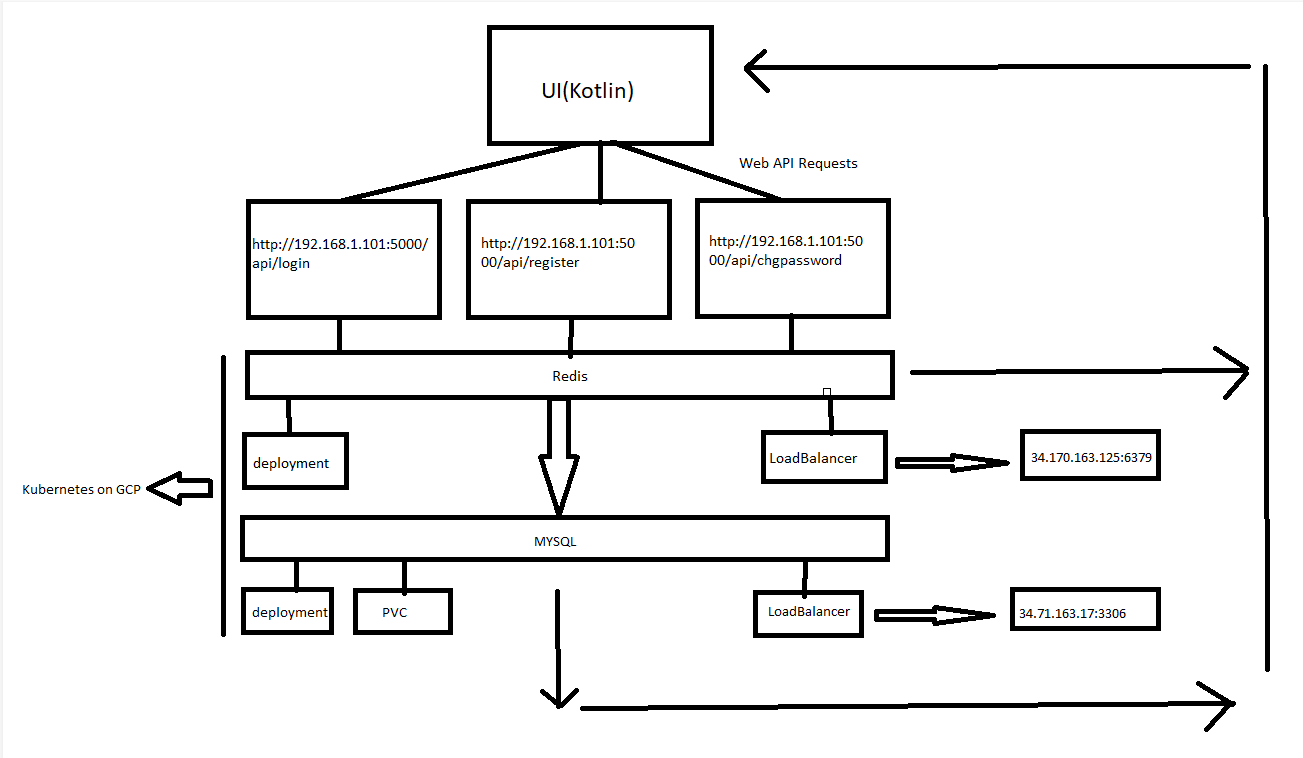
\includegraphics[scale=0.27]{Yazlab3LoginARCH.png}
    \caption{Uygulama Mimarisi}
    \label{fig:spark}
\end{figure}

    
\end{itemize}
\section{Pseudo Kod(Kabakod)}

1. Giriş ekranı gelir.\\
2. Eğer kullanıcı adı ve şifre girerse bunları apiye ilet cevaba göre onayla veya alert dön.\\
3. Eğer şifre unuttuma basarsa git. Eski şifresini ve yeni şifresini al. Apiye yolla. Api cevabına göre şifreyi değiştir.\\
4. Yeni kullanıcı oluşturmak istiyorsa git. Bilgileri al.Kaydet apiye yolla. Apide kayıt işlemini gerçekleştir. Response dön.\\
5. Kullanıcı başarılı bir şekilde giriş yaparsa oyun tercihleri yapacağı sayfayı getir.\\
6. Kullanıcıdan tercihleri iste. Her tercihi girdikten sonra ilgili oyunu CardAPI'sine giderek kart bilgilerini çek.\\
- O ara kullanıcıya SplashScreen'i göster.
7. Cardları kotlin üzerinde spesifik bir class'a çek. Sonrasında kartları shufflela.\\
8. Her bir butonu kart bilgileriyle eşleştir.\\
9. Timer'i başlatarak oyunu başlat. Oyun başladığı anda müziği de çal.\\
10. Eğer kullanıcı doğru eşleşme yaparsa ilgili müziği çal. Kazandırdığı puanı hesapla. Arayüzde göster.\\
11. Eğer kullanıcı yanlış eşleşme yaparsa kaybettiği puanı hesapla. Skorundan çıkar. Bastığı kart bilgisini textview olarak ScrollBar'a ekle.\\ 
12. Süreyi sürekli kontrol et. Tüm kartlar eşleşmeden süre bittiyse kaybettin yaz ve kaybettin müziğini çaldır.\\
13. Süre bitmeden kartlar eşleştirilmişse kazandın yaz ve kazandın müziğini çal.\\
14. Oyun bittiğinde kullanıcıyı ana menüye dön ve tekrar oyna olarak 2 butonla karşıla.\\
15. Bu döngüye sürekli böyle devam et.\\    






\section{Sonuç}

Bu projede birçok kazanım elde ettik. Ayrıca birçok sorunla karşılaştık. Bu durumun bizi oldukça geliştirdiğini öğrendik.\\
Elde ettiğimiz kazanımlardan bahsedecek olursak;\\

\begin{itemize}
    \item Android Studio ortamını öğrenmek,
    \item Kotlin ile yazılım geliştirmeyi öğrenmek,
    \item Event Listener yapılarını kullanmayı öğrenmek,
    \item Bulut platformunu öğrenmek,
    \item Veri tabanı CRUD işlemlerini öğrenmek,
    \item API ile farklı diller arasında veri akışı sağlamayı öğrenmek,

\end{itemize}

Kazanımlarını elde ettik.\\

\section{Kaynakça}

\begin{itemize}
    \item 
    https://medium.com/kodlayan-nesil/flask-nedir-9364c1bb5f41
    \item https://aws.amazon.com/tr/what-is/api/
    \item https://kotlinlang.org/
    \item https://developer.android.com/studio
    \item https://github.com/
    \item https://www.btkakademi.gov.tr/portal/course/kotlin-ile-android-mobil-uygulama-gelistirme-egitimi-temel-seviye-10274
    \item https://bilgisayarkavramlari.com
    \item https://medium.com/@ecemsuren/kotlin-temelleri-2c9ad608af7d
    \item https://stackoverflow.com/
    \item https://www.protan.com.tr/mysql-nedir/
    \item .https://devnot.com/2020/redis-nedir-temel-kullanim-alanlari-nelerdir/
    \item https://deniz-turkmen.medium.com/dockerfile-a177c7796d53
    \item https://www.google.com/url?sa=i&url=https%3A%2F%2Fdzone.com%2Farticles%2Fredis-vs-mysql-benchmarks&psig=AOvVaw0HCW1iKDOTMFCijNFw9St4&ust=1671477366666000&source=images&cd=vfe&ved=0CA0QjRxqFwoTCMDKpMjwg_wCFQAAAAAdAAAAABAD
    

\end{itemize}

\section{Deneysel Sonuçlar}

\begin{figure}[ht] 
    \centering
    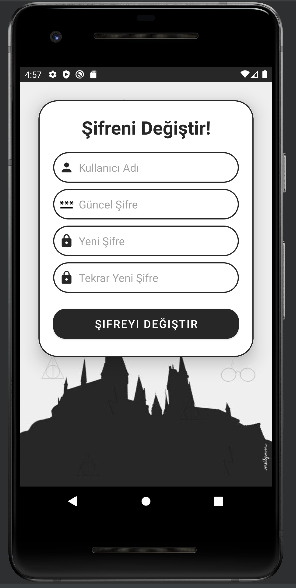
\includegraphics[scale=0.35]{changePass.png}
    \caption{Şifre Değiştirme Ekranı}
    \label{fig:spark}
\end{figure}
\begin{figure}[ht] 
    \centering
    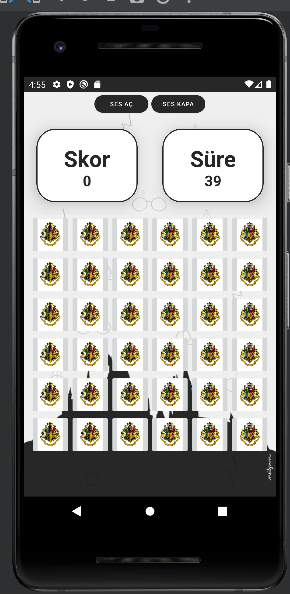
\includegraphics[scale=0.35]{game.png}
    \caption{Oyundan Bir Görüntü}
    \label{fig:spark}
\end{figure}
\begin{figure}[ht] 
    \centering
    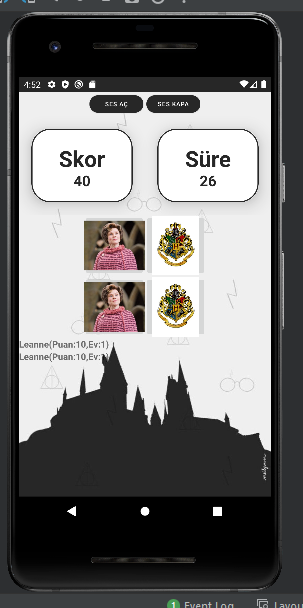
\includegraphics[scale=0.35]{game2.png}
    \caption{Oyundan Bir Görüntü}
    \label{fig:spark}
\end{figure}

\begin{figure}[ht] 
    \centering
    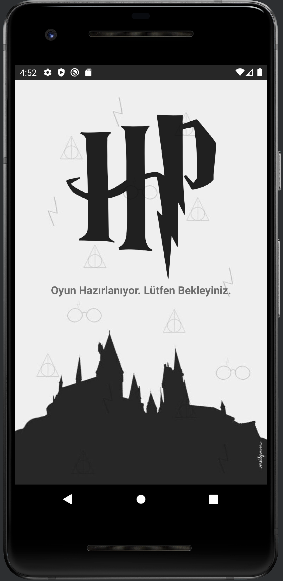
\includegraphics[scale=0.35]{loading.png}
    \caption{Yükleme Ekranı}
    \label{fig:spark}
\end{figure}
\begin{figure}[ht] 
    \centering
    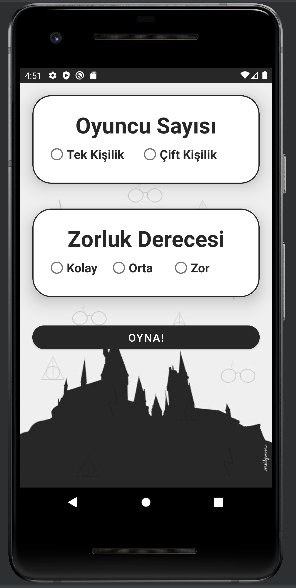
\includegraphics[scale=0.35]{mainmenu.png}
    \caption{Ana Menü}
    \label{fig:spark}
\end{figure}
\newpage

\end{document}